\section{\textbf{INDUKTIVE STATISTIK} - Parameterschätzung}
Maßzahlen, wie Mittelwerte oder die Stichprobenvarianz bestimmt nach um aussagen über die die konkreten Beobachtung innerhalb der Stichprobe zu treffen sondern als \emph{Schätzer} für \underline{nicht} beobachtbare Größen der zugrundeliegenden Grundgesamtheit bzw. Population.
\subsection{Schätzstatistiken und Schätzwerte}
Punktschätzung: Beschreiben von einer Eigenschaft oder Parameter einer Grundgesamtheit mittels eines einzigen Näherungswertes. Beispielsweise von der Varianz oder dem Erwartungswert.
Den für die Grundgesamtheit zu schätzende Parameter wird idr mit $\theta$ bezeichnet. Die Schätzung von $\theta$ erfolgt dann mit Hilfe einer Funktion in Abhängigkeit von den Beobachtungen innerhalb einer Stichprobe, der sogenannten \emph{Schätzfunktion, Schätzstatistik} oder kurz \emph{Schätzer}: $T = g(X_1, ..., X_n)$. Die Schätzstatistik $T$ ist hierbei selbst wieder eine Zufallsvariable. Der \emph{Schätzwert}, der sich aus den Realisierungen der einzelnen Zufallsvariablen $X_i$ ergibt wird mit $t = g(x_1, ..., x_n)$ bezeichnet. Beispiele für Schätzer sind die Lagemaße und kenndaten von Stichproben aus vorangegangen Abschnitten.
\subsection{Eigenschaften von Schätzstatistiken}
\hlc{Erwartungstreue}: Ein Schätzer $T$ wird als erwartungstreu bezeichnet, 
wenn er im Erwartungswert genau den Wert $\theta$ liefert, den sie schätzen soll: $E(T) = E(g(X_1, ..., X_n)) = \theta$. Ist eine Schätzstatistik $T$ nicht erwartungstreu, 
so misst man die systematische Über- oder Unterschätzung mit dem \hlc{Bias}: 
$Bias(T) = E(T) - \theta$. Beispielhafte Rechnung für die \hlc{empirische Varianz} 
$\overset{\sim}{S}^2 = \frac{1}{n} \sum_{i=1}^{n}(X_i - \bar{X})^2 = \frac{n - 1}{n}S^2$: 
$Bias(\overset{\sim}{S}^2) = E(\overset{\sim}{S}^2) - \sigma^2 = \frac{n - 1}{n}\sigma^2 - \sigma^2 = - \frac{\sigma^2}{n}$. 
Da $\underset{n \rightarrow \infty}{lim} E(T) = \theta$ gilt spricht man hierbei von einer \emph{asymptotisch erwartungsgetreuen} Schätzstatistik. 
Das hingegen arithmetische Mittel ist ein erwarungstreuer Schätzer 
$E(\bar{X}) = \frac{1}{n}\sum_{i=1}^{n}E(X_i)=\frac{1}{n}n\mu = \mu$. 
Der \hlc{Standardfehler} des arithmethischen Mittels für unabhängige Beobachtungen ist jedoch: 
$\sigma_{\bar{X}} = \sqrt{Var(\frac{1}{n} \sum_{i=1}^{n}X_i)} = \sqrt{\frac{1}{n^2}\sum_{i=1}^nVar(X_i)} = \sqrt{\frac{1}{n^2}n\sigma^2} = \frac{\sigma}{\sqrt{n}}$\\\\
\hlc{Mittlere quadratische Abweichung}: $MSE(T) = E((T - \theta)^2) = Var(T) + Bias^2(T)$ eine Schätzstatistik $T$
bezeichnet man als \hlc{konsistent} (im quadratischen Mittel), wenn gilt: $MSE(T) \rightarrow 0$ für $n \rightarrow \infty$.
Der $MSE$ eignet sich auch gut für den Vergleich von Schätzstatistiken. Die Schätzstatistik, mit kleineren $MSE$,
wird als \emph{wirksamer} oder \emph{effizienter} bezeichnet. 
\subsection{Konstruktion von Schätzstatistiken}
\hlc{Momente-Methode}: Man schätzt verteilungsspezifisch parameter mit dem z.B. dem Erwartungswert. Bsp. für $Pos(\lambda)$
$E(X) = \lambda$. Analog können auch $\mu$ und $\sigma^2$ einer Normalverteilung mit Hilfe des arithmetischen Mittels und der Stichprobenvarianz geschätzt werden.
\hlc{Kleinste Quadrate Methode}: Geeignet für die Parameter einer Regressionsgerade (siehe Regression) aber auch für $\mu$ ein mögliche Schätzstatistik
für den Erwartungswert wäre: $T = \underset{z}{\text{arg min}}\sum_{i=1}^{n}(X_i - z)^2$.\\\\
\hlc{Maximum-Likelihood-Schätzung (ML-Schätzer)}: Ein verfahren, bei dem Vorwissen oder eine Annahme zu Verteilung voraussetzt. 
Idee: wähle Schätzwert für Parameter so, dass die Wahrscheinlichkeit, die Realisierung einer konkreten Stichprobe zu beobachten, maximiert wird.
Formal wird hier mit $f(x|\theta)$ die Wahrscheinlichkeitsfunktion bzw. Wahrscheinlichkeitsdichte einer Verteilung bezeichnet. 
Beispiel für $Pos(\lambda)$: $f(x|\lambda) = \frac{\lambda^x}{x!}e^{-\lambda}$ oder $N(\mu, \sigma^2)$: $f(x|\mu, \sigma) = \frac{1}{\sqrt{2\pi}\sigma}e^{-\frac{(x-\mu)^2}{2\sigma^2}}$
Diese Funktion soll nach dem Maximum-Likelihood-Prinzip bzglch. $\theta$ maximiert werden. 
Die zu optimierende Funktion $L(\theta) = f(x_1, ..., x_n|\theta)$ wird als \hlc{Likelihoodfunktion} bezeichnet.
Die Schätzstatistik $\hat{\theta} = \hat{\theta(x_1, ..., x_n)}$ mit 
$L(\hat{\theta}) = \underset{\theta}{\text{max}}L(\theta) = \underset{\theta}{max}f(x_1, ..., x_n|\theta)$ bezeichnet man als Maximum-Likelihood Schätzer oder (ML Scätzer) für den unbekannten Parameter(vektor) $\theta$.
Sind die einzelnen Realisierungen unabhängig gilt $L(theta) = f(x_1|\theta) \cdot ... \cdot f(x_n|\theta)$
Bsp: \hlcm{$Pos(\lambda)$: $L(\lambda) = \Pi_{i=1}^n\frac{\lambda^{x_i}}{x_i!}e^{-\lambda}$}. Die \hlc{Loglikelihoodfunktion} ergibt sich durch $l(\theta) = \text{ln}L(\theta) = ln(\Pi_{i=1}^nf(x_i|\theta)) = \sum_{i=1}^nln(f(x_i|\theta))$ (unabhängig vorausgesetzt). Die optimierung dieser Funktion ist einfacher und die Monotonie des Logs garantiert Maxima an den gleichen stellen.
Bsp: \hlcm{$Pos(\lambda)$: $L(\lambda) = \sum_{i=1}^n\text{ln}(\frac{\lambda^{x_i}}{x_i!}e^{-\lambda}) = \sum_{i=1}^{n}\text{ln}(\lambda^{x_i}) - ln(x_i!) + ln(e^{-\lambda}) = ln(\lambda)\sum_{i=1}^{n}x_i - \sum_{i=1}^{n}ln(x_i!) - n\lambda$} $\rightarrow$ 
Ableiten und null setzen: $l'(\hat{\lambda}) = \frac{1}{\hat{\lambda}}\sum_{i=1}^{n}x_i - n = 0 \Leftrightarrow \hat{\lambda}=\frac{1}{n}\sum_{i=1}^{n}x_i=\bar{x}$
\subsection{Konfidenzintervalle}
\begin{wrapfigure}{l}{0.5\textwidth}
    \vspace{-5mm}
    \centering
    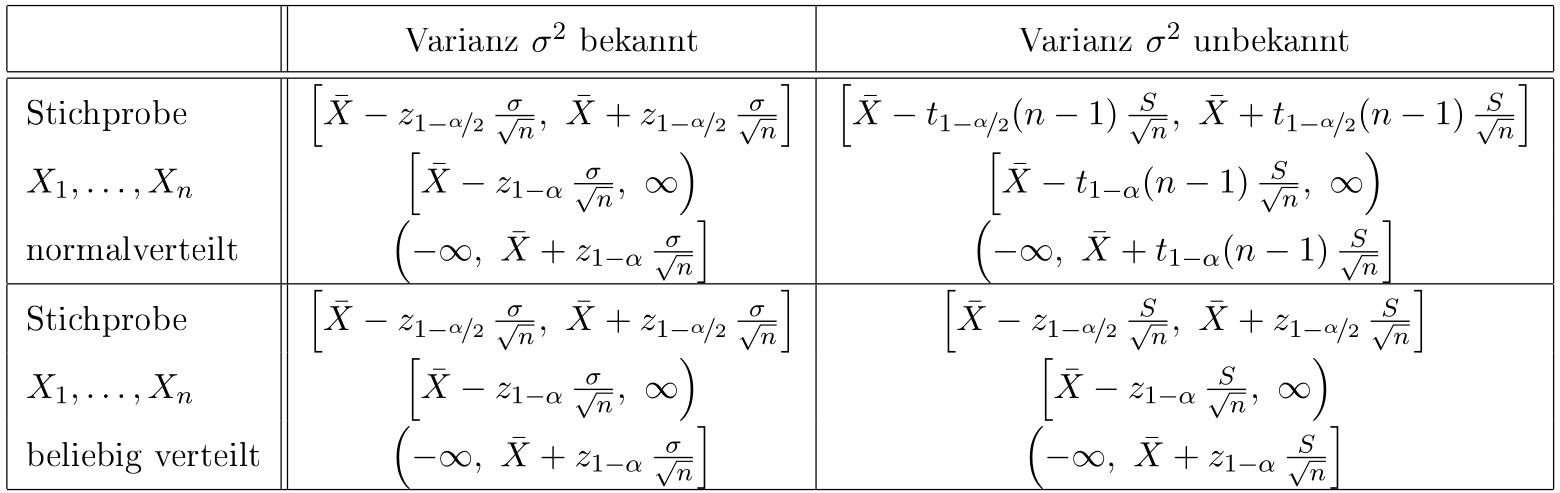
\includegraphics[width=0.5\textwidth]{images/tab9.1_konfidenzintervalle.png}
    \caption{Zweiseitige und einseitige $(1 - \alpha)$ -Konfidenzintervalle unter verschiedenen Verteilungsannahmen für
    die Stichprobenvariablen sowie bei bekannter und unbekannter Varianz}
    \vspace{-10mm}
    \label{fig:konfi}
\end{wrapfigure}
Alternative zur Punktschätzung, bei der man nicht einen Schätzwert für einen Parameter bestimmt, sondern ein Intervall, in dem der Parameter einer vorgegebenen Wahrscheinlichkeit liegt.
\hlc{Zweiseitige Konfidenzintervalle}: Dafür werden zwei Schätzstatistiken benötigt: $G_u = g_u(X_1, ... X_n)$ und $G_o = g_o(X_1, ... X_n)$.
Die \hlc{Irtumswahrscheinlichkeit $\alpha$} gibt an, mit welcher Wahrscheinlichkeit der Parameter außerhalb des Intervalls liegt $P(G_u \le \theta \le G_o) = 1 - \alpha$. Schreibweise für Stichprobe $x_1, ... x_n$: $[g_u, g_o] = [g_u(x_1, ..., x_n), g_o(x_1, ..., x_n)]$ (Konkrete grenzen, und $\theta$ ist drin oder eben nicht). \hlc{einseitige Konfidenzintervalle}: Wenn z.B. die obere Grenze unendlich ist: $[g_u, \infty)$\\\\
\hlc{Konfidenzintervalle für den Erwartungswert} vgl: \cref{fig:konfi} \\\\
\hlc{Konfidenzintervalle für Eintrittswahrscheinlichkeiten}: Intervallschätzung für die Eintrittswahrscheinlichkeit $p$ eines bestimmten Ereignisses $A$ bei $n$ unabhängigen Wiederholungen.
Die $Bin(n,p)$- verteilte Summe $X = X_1 + ... + X_n$ ist bei hinreichend großen $n$ normalverteilt mit $E(X) = np$ $Var(X) = np(1-p)$. Somit gilt $\bar{X} \sim N(p, \frac{p(1-p)}{n})$ bzw. $\frac{\bar{X} - p}{\sqrt{\frac{p(1-p)}{n}}}\sim N(0,1)$. 
Das Approximierte $(1 - \alpha)$-Konfidenzintervall ist $[\bar{X} - z_{1 - \frac{\alpha}{2}}\sqrt{\frac{\bar{X}(1-\bar{X})}{n}}, \bar{X} + z_{1 - \frac{\alpha}{2}}\sqrt{\frac{\bar{X}(1-\bar{X})}{n}}]$ bzw. die einseitigen Konfidenzintervalle, wenn $p \in (0, 1)$: $[\bar{X} - z_{1 - \frac{\alpha}{2}}\sqrt{\frac{\bar{X}(1-\bar{X})}{n}}, 1)$ und $(0, \bar{X} + z_{1 - \frac{\alpha}{2}}\sqrt{\frac{\bar{X}(1-\bar{X})}{n}}]$

\section{Signifikanztests}
Mögliche Fragestellung: ab wie vielen defekten Teilen in einer Stichprobe der Größe $n$ ist die Angabe einer Höchstausschusrate $p$ falsch, wenn man die Aussage nur mit $\alpha$ anzweifeln möchte?\\\\
\hlc{Vorgehen}:
\begin{enumerate}[leftmargin=*]
    \itemsep0em 
    \item Quantifizierung des inhaltlichen Problems: Die Problematik defekter Teile wurde mit Hilfe der Ausschussrate Quantifiziert. Also $n \cdot p$
    \item Formulierung der Modellannahme. Kann man davon ausgehen, dass die Stichprobenvariablen unabhängig, identisch bzw. einer eindeutigen Verteilung angehören? Wenn ja $\rightarrow$ parametrischer Test, da man gg. Parameter testen kann. Anderenfalls nichtparametrischer Test und man muss ohne auskommen.
    \item Aufstellen der testenden \emph{Nullhypothese} $H_0$ und der Alternativhypothese $H_1$. Bei einseitigen Testproblemen ist die Abweichung in nur eine Richtung interessant: $H_0: p \le 0.005$ vs $H_1: p > 0.05$. Bei Hypothesen der Form $H_0: \theta = c$ vs. $H_1 \theta \neq c$ spricht man von Zweiseitigen Testproblemen.
    \item Wahl einer geeigneten Teststatistik. Für ein Problem wie mit defekten Teilen könnte man sowas wie $X = X_1 + ... + X_60$ wählen. Allgemein also einfach eine Funktion, die alle Stichprobenvariablen beinhaltet.
    \item Identifikation der Testverteilung. Wähle Teststatistik so, dass sie unter Annahme das $N_0$ korrekt ist einer bekannten Wahrscheinlichkeitsverteilung folgen. Wähle bei einseitigen die Parameter so, dass sie möglichst nah an $N_1$ liegen.
    \item Festlegung des Signifikanzniveaus $alpha$: Mit welcher Wahrscheinlichkeit ist man bereit $N_0$ zu verwerfen, obwohl sie korrekt ist. Typische Werte sind $1\%$, $5\%$ $10\%$.
    \item Bestimmung des Ablehnungsbereichs. Der Ablehnungsbereichs enthält alle werte der Teststatistik $T$, für die die $H_0$ abgelehnt wird und $H_1$ deutlich plausibler wird. Dieser Bereich wird durch von $\alpha$ abhängige Quantile festgelegt. Im einseitigen Test von z.B. einer Eingangskontrolle mit $\alpha = 5\%$ nutzt man $95\%$-Quantil von einer $Bin$-verteilung. Für $Bin(60, 0.05)$ wäre das $A = {6, 7, ... 60}$. Das Komplement von $A$ ist der Annahmebereich.
    Bei Zweiseitigen Testproblemen besteht der Ablehnungsbereichsbereich idR aus zwei Teilen, da sowohl sehr große als auch sehr kleine Werte der Teststatistik kritisch sind. In dem Fall teilt man die Irrtumswahrscheinlichkeit $\alpha$ in zwei Hälften auf: $A = \{t: t<q_{\alpha/2}\} \cup \{t: t>q_{1 - \alpha/2}\}$. die beiden $q$ sind hierbei die $\alpha/2$ bzw $(1 - \alpha/2)$-Quantile.
    \item Berechnung der Teststatistik. 
    \item Entscheidung. Prüfe, in welchen Bereich das Ergebnis liegt 
\end{enumerate}
\hlc{Fehler 1. Art}: $H_0$ wahr aber verworfen. Es gilt $P(\text{Fehler 1. Art}) = P(H_0 \text{verwerfen} | H_0 \text{wahr}) \le \alpha$ \hlc{Fehler 2. Art}: $H_0$ falsch aber beibehalten.$P(\text{Fehler 2. Art}) = P(H_0 \text{beibehalten} | H_0 \text{falsch})$ 
\subsection{Ein-Stichproben-Testprobleme}
\hlc{Der (approxmierte) Binomialtest}: 
\subsection{Mehr-Stichproben-Testprobleme}
\subsection{Der $\chi^2$-Unabhängigkeitstest}